
\chapter{A prototypical model of an ion channel \label{prototype}}

So far we have been concerned with calcium-induced calcium release (CICR) as
illustrated in Figure \ref{geomCa_V} (page \pageref{geomCa_V}). To
study CICR, we started by studying the development of the concentration of
calcium ions in the dyad and kept everything else constant. The interesting
part was then to see how the release mechanism of the ryanodine receptor RyR changes 
the dynamics of the dyad concentration. In particular, we were interested in RyR 
mutations and their theoretical effect on the dyad concentration through changes in the
open probability of the RyR channel. We saw how theoretical blockers could be
defined in order to repair the effect of the mutations, in the sense that we
were able to restore essential properties of the process. We also introduced the
effect of allowing the concentration of the junctional sarcoplasmic reticulum 
 to change and we studied how the overall processes were affected by introducing 
 the transmembrane potential and allowing the L-type calcium channel (LCC) to open and close. 

Now we leave the RyR and Markov
models based on concentrations of calcium ions and focus on
voltage-gated channels. We touched upon this topic earlier, since the LCC
is voltage gated, but now we will dynamically update the voltage and focus
solely on how voltage develops and how it affects the transitions of the
Markov model.

We will start by studying a very simple channel to explain
the basics steps as carefully as possible. This channel does not have a name and
probably does not exist in nature, but it provides a good example to
get a handle on the steps involved in understanding much more complex (and more
realistic) ion channels. 
%In later chapters we will focus on both Sodium and Potassium channels and study theoretical drugs for these channels.

In the study of CICR, we examined what was going on in a very small part of the 
cell based on the tacit assumption that if we can repair what is going on in 
every tiny part of the cell, we will probably also do a decent job in repairing all of the cell. We will follow the same strategy in studying voltage-gated channels: We will study a single channel and see how mutations may affect the 
function of the channel and thereby how the transmembrane potential is changed. Again, we will derive 
theoretical drugs and see how they should be defined in order to repair the effect of the mutations. However, the assumption that small domains can be studied independently is less reliable for voltage-gated channels than for 
the CICR process in the vicinity of the dyad. The reason for this is that electrical diffusion waves travel much faster than concentration waves. %Therefore we will conclude our analysis of voltage-gated ion channels by adding many of them together and study the whole cell effect of the theoretical drugs we propose. This will be done in Chapter \ref{ap}, but first we will spend some time studying single channels.

\section[Stochastic model]{Stochastic model of the transmembrane potential}

The transmembrane potential is defined to be the difference between the
intracellular potential $v_{i}$ and the extracellular potential $v_{e}$:%
\begin{equation}
v=v_{i}-v_{e}. \label{v0}%
\end{equation}
Let us consider a membrane consisting of a leakage current with conductance
given by $g_{L}$ and an ion channel with conductance given by $g_{i}.$ The
transmembrane potential of such a membrane is governed by the
differential equation%
\begin{equation}
Cv^{\prime}=-g_{L}\left(  v-V_{L}\right)  -g_{i}(v-V_{i}), \label{v1}%
\end{equation}
where $C$ is the capacitance of the membrane, $V_{L}$ is the resting potential
of the leakage current, and $V_{i}$ is the resting potential of the ion
channel. In our computations, we will consider an example\footnote{Here, the choice of the parameter $V_i$ may seem a bit strange, but we will see below that it will lead to a very simple computational domain for the probability density functions.} 
with the parameters listed in Table \ref{11on10}.
\graytable{l}{
{|c|c|} \hline
$C$ &  $1$ $\mu\text{F/cm}^{2}$\\ \hline
$g_L$ & $1/10 \text{ mS/cm}^{2}$ \\ \hline
$V_L$ & $0\text{ mV}$ \\ \hline
$V_{i}$ & $11/10\text{ mV}$\\ \hline
}{ Values of the parameters used in the model \ref{v1}.\label{11on10}}
%\begin{align*}
%C  &  =1 \text{ } \mu\text{F/cm}^{2},\\
%g_{L}  &  =\frac{1}{10}\text{ mS/cm}^{2},\\
%V_{L}  &  =0\text{ mV,}\\
%V_{i}  &  =\frac{11}{10}\text{ mV.}%
%\end{align*}
We assume that the ion channel can be either open (O), with $g_{i}=1$ mS/cm$^{2},$ or
closed (C), with $g_{i}=0$ mS/cm$^{2}$. The state of the stochastic ion channel is governed
by a Markov model of the form%
\begin{equation}
C\underset{k_{co}}{\overset{k_{oc}}{\leftrightarrows}}O, \label{Markov_volt}%
\end{equation}
where the reactions rates will be specified below. With these definitions, the
stochastic equation takes the form%
\begin{equation}
v^{\prime}=-\frac{1}{10}v-\gamma\left(  v-\frac{11}{10}\right),  \label{v2}%
\end{equation}
where $\gamma$ is zero (closed) or one (open) depending on the state of the Markov model (\ref{Markov_volt}).

\subsection{A numerical scheme}

We compute numerical solutions of the model $\left(  \ref{v2}\right)  $ using
the scheme%
\begin{equation}
v_{n+1}=v_{n}-\Delta t\left(  \frac{1}{10}v_{n}+\gamma_{n}\left(  v_{n}%
-\frac{11}{10}\right)  \right)  \label{vs},%
\end{equation}
where $\Delta t$ denotes the time step and $\gamma_{n}$ takes on values
based on the state of the Markov model. Based on the Markov model, the value
of $\gamma_{n}$ is computed as described on page \pageref{numscheme}. We assume that
the time step (in ms) satisfies the condition%
\begin{equation}
\Delta t<\frac{10}{11}. \label{vdt}%
\end{equation}



\subsection{An invariant region}

We discussed above that it is useful to derive an invariant region for the
stochastic model since such a region can be used to define the computational
domain of the probability density equation. We claim that, under the condition
$\left(  \ref{vdt}\right)  $ for the time step, the solutions generated by 
scheme $\left(  \ref{vs}\right)  $ will always remain in the interval given by%
\[
\Omega=(0,1),
\]
provided that the initial condition is in this region. To show that
$\Omega$ is an invariant region for solutions generated by scheme $\left(
\ref{vs}\right)  $, we write the scheme in the form%
\[
v_{n+1}=H(v_{n},\gamma_{n}),
\]
where%
\[
H(v,\gamma)=v-\Delta t\left(  \frac{1}{10}v+\gamma\left(  v-\frac{11}%
{10}\right)  \right)  .
\]
Since%
\[
\frac{\partial H(v,\gamma)}{\partial v}=1-\Delta t\left(  \frac{1}{10}%
+\gamma\right)  >0
\]
because of $\left(  \ref{vdt}\right) $ and%
\[
\frac{\partial H(v,\gamma)}{\partial\gamma}=\Delta t\left(\frac{11}{10}-v\right)>0
\]
for any $v\in\Omega,$ we have%
\[
v_{n+1}=H(v_{n},\gamma_{n})\leqslant H\left(  1,1\right)  =1
\]
and%
\[
v_{n+1}=H(v_{n},\gamma_{n})\geqslant H(0,0)=0.
\]
So, by induction, we have  $v_{n}\in\Omega$  for all $n$.



\section[Probability density functions]{Probability density functions for the voltage-gated channel}

We can now follow exactly the same steps as in Section \ref{sec:pdf} (see page
\pageref{sec:pdf}) to derive a model of the probability density
functions of the open state and the closed state. The probability of the
channel being in the open state for voltages between $v$ and $v+\Delta v$ is
given by%
\[
P_{o}\left\{  v<V(t)<v+\Delta v\right\}  =\int_{v}^{v+\Delta v}\rho_{o}(w,t)dw,
\]
where $\rho_{o}$ is the probability density function of the open state.
Similarly, we have%
\[
P_{c}\left\{  v<V(t)<v+\Delta v\right\}  =\int_{v}^{v+\Delta v}\rho_{c}(w,t)dw
\]
where $\rho_{c}$ is the probability density function of the closed state. By
the arguments given in Section \ref{sec:pdf}, we find that the probability
density functions must be solutions of the system%
\begin{align}
\frac{\partial\rho_{o}}{\partial t}+\frac{\partial}{\partial v}\left(
a_{o}\rho_{o}\right)   &  =k_{co}\rho_{c}-k_{oc}\rho_{o},\label{vpdf}\\
\frac{\partial\rho_{c}}{\partial t}+\frac{\partial}{\partial v}\left(
a_{c}\rho_{c}\right)   &  =k_{oc}\rho_{o}-k_{co}\rho_{c},\nonumber
\end{align}
where the flux terms are given by
\begin{align}
a_{o} &  =-g_{L}\left(  v-V_{L}\right)  -(v-V_{i})=\frac{11}{10}\left(
1-v\right)  ,\label{vflux}\\
a_{c} &  =-g_{L}\left(  v-V_{L}\right)  =-\frac{1}{10}v\nonumber
\end{align}
%\K{zzz Skal man egentlig dele p\r{a}  C i uttrykkene for $a_o$ og $a_c$ eller blir C-en bakt inn i ligningen p\r{a}  en annen m\r{a}te?}
%\A{In principle, yes, but since C=1, we do nothing (except that we changes units)}

%\KHJ{I dette kapittelet og de neste brukes b\aa de $V$ og $v$ om spenningen.  Er det noe system p\r{a} n\aa r man bruker hva eller er det bare tilfeldig?}

As usual, the boundary conditions are set up to avoid a probability leak
across the boundary. Hence we need the  fluxes $a_{o}\rho_{o}$ and
$a_{c}\rho_{c}$ to be zero for $v=0$ and $v=1.$ Note that $a_{o}%
(1)=a_{c}(0)=0;$ so we require $\rho_{o}(0)=0$ and $\rho_{c}(1)=0.$ In
the numerical simulations presented below, we use the scheme described in
Section \ref{npdf}. Stationary solutions of the numerical scheme are computed
as described on page \pageref{accuracy}.


\section{Analytical solution of the stationary case}

We showed in Section \ref{sec:analytical} how an analytical solution can be derived
for a stationary system of the form $\left(  \ref{vpdf}\right)  .$ Here we
shall repeat this derivation for a voltage-gated channel. For simplicity we
shall consider a channel where the reaction scheme of the Markov model is
independent of the voltage; we choose%
\[
k_{oc}=1\text{ ms}^{-1}\text{ and }k_{co}=\mu\text{ ms}^{-1}.
\]
So, we will again focus on CO-mutations.
Here $\mu$, referred to as the mutation severity index,
 will be specified in the computations below.  In all computations, $\mu=1$ will be 
 referred to as the wild type case. Increased values of
$k_{co}$ will increase the open probability of the ion channel in $\left(
\ref{v1}\right)  $ and therefore bring the transmembrane potential closer to
the maximum  value (given by $V_{+}=1$ mV). 

The first step in the derivation of the analytical solution is to observe that, in the
steady state, the sum of the equations of $\left(  \ref{vpdf}\right)  $ results
in the equation%
\[
\frac{\partial}{\partial v}\left(  a_{o}\rho_{o}+a_{c}\rho_{c}\right)  =0.
\]
The second step is to observe that the boundary conditions imply that%
\[
a_{o}\rho_{o}+a_{c}\rho_{c}=0.
\]
Therefore, for the present model, we find that%
\[
\rho_{c}=-\frac{a_{o}}{a_{c}}\rho_{o}=\frac{11}{v}\left(  1-v\right)  \rho_{o}%
\]
and, from $\left(  \ref{vpdf}\right)  $, we have
\[
\frac{\partial}{\partial v}\left(  a_{o}\rho_{o}\right)  =\mu\rho_{c}-\rho
_{o}=\left(  11\mu\frac{1-v}{v}-1\right)  \rho_{o}.
\]
By differentiation, we obtain%
\[
a_{o}\frac{\partial}{\partial v}\rho_{o}=\left(  11\mu\frac{1-v}{v}%
-1-\frac{\partial}{\partial v}a_{o}\right)  \rho_{o}%
\]
and thus%
\begin{equation}
\rho_{o}^{\prime}=a(v)\rho_{o}, \label{rho1}%
\end{equation}
where%
\[
a(v)=\left(  \frac{10\mu}{v}+\frac{1}{11(1-v)}\right)  .
\]
The solution of $\left(  \ref{rho1}\right)  $ is given by%
\begin{equation}
\rho_{o}=c\frac{v^{10\mu}}{\left(  1-v\right)  ^{1/11}}\label{rho2}%
\end{equation}
and then%
\[
\rho_{c}=11 c \left(  1-v\right)  ^{10/11}v^{10\mu-1}.
\]
Here the constant $c$ must be chosen such that%
\[
\int_{\Omega}\left(  \rho_{o}+\rho_{c}\right)  dv=1.
\]

It is interesting to note here that, even if both $\rho_o$ and $\rho_c$ depend heavily on the mutation severity 
index $\mu$, the relation between these functions is independent of $\mu$ since
\[ \frac{\rho_o}{\rho_c}=\frac{v}{11(1-v)}. \]

\section[Comparison of MCs and PDFs]{Comparison of Monte Carlo simulations and probability density functions}


In previous chapters we gave many examples showing that the probability density
functions faithfully represent the frequency distributions that can be
computed using Monte Carlo simulations. We will briefly show that this also
holds for the ion channel model considered here. In Figure \ref{V/mc_mut.pdf}, we compare the
open probability density function given by $\left(  \ref{rho2}\right)  $ and a
histogram computed using Monte Carlo simulations based on the numerical scheme
given by $\left(  \ref{vs}\right)  .$  We observe again---and by now we are starting to get used to it---that the probability density functions 
more or less coincide with the histograms computed using Monte Carlo simulations.\footnote{At this point
it feels appropriate to remind the reader of one of the many great quotes by John von Neumann: 
{``In mathematics you don't understand things. You just get used to them.''}
}

\fig{V/mc_mut.pdf}{Comparison of the results of Monte Carlo simulations (histogram) and 
analytical solutions of the system
governing the probability density functions for four values of the mutation severity 
index $\mu$. The unit interval is divided into 100 sub-intervals where the 
number of occurrences is counted in the Monte Carlo simulations. The analytical solutions are evaluated in the center of these sub-intervals. Each case was simulated for 10 s, with $\Delta t=0.01$ ms.}


\section{Mutations and theoretical drugs}

In our analysis of the RyR, we studied the effect of mutations increasing the 
open probability of the channel. In addition, for voltage-gated ion
channels, mutations may affect the open probability of the channel and thereby
change the dynamics of the transmembrane potential. We will study specific
examples of this below, where we present actual mutations and their effect on
actual ion channels, such as the sodium channel. However, for the time being,
we will stick to our not so realistic but rather cute model. We will assume 
that the stochastic dynamics of the transmembrane potential are governed by 
$\left(\ref{v1}\right)$,  that the probability density functions are governed by
$\left(  \ref{vpdf}\right)$, and that the Markov model is given by%
\begin{equation}
C\underset{k_{co}}{\overset{k_{oc}}{\leftrightarrows}}O,
\end{equation}
where $k_{oc}=1 \text{ ms}^{-1}$ and $k_{co}=\mu\text{ ms}^{-1}.$ 
As usual,  $\mu$ is the mutation severity
index and $\mu=1$ denotes the wild type case. 
Motivated by the results for the RyR mutations,
we will try to repair the effect of the mutation using an open or a closed
state blocker. This will prove to be quite efficient, since we are dealing with a CO-mutation.

\bigskip

\subsection{Theoretical open state blocker}

The Markov model of the theoretical open state blocker is%
\begin{equation}
C\underset{k_{co}}{\overset{k_{oc}}{\leftrightarrows}}O\underset{k_{ob}%
}{\overset{k_{bo}}{\leftrightarrows}}B, \label{ob1}%
\end{equation}
where the parameters $k_{bo}$ and $k_{ob}$ need to be determined. The
associated steady state version of the probability density system is given by%
\begin{align}
\frac{\partial}{\partial v}\left(  a_{o}\rho_{o}\right)   &  =k_{co}\rho
_{c}-\left(  k_{oc}+k_{ob}\right)  \rho_{o}+k_{bo}\rho_{b},\nonumber\\
\frac{\partial}{\partial v}\left(  a_{c}\rho_{c}\right)   &  =k_{oc}\rho
_{o}-k_{co}\rho_{c},\label{osb1}\\
\frac{\partial}{\partial v}\left(  a_{c}\rho_{b}\right)   &  =k_{ob}\rho
_{o}-k_{bo}\rho_{b},\nonumber
\end{align}
where $\rho_{o},\rho_{c},$ and $\rho_{b}$ denote the probability density
functions of the open (O), closed (C), and blocked (B) states, respectively. We
compute optimal values of the parameters $k_{bo}$ and $k_{ob}$ using the
{\it Fminsearch} function in Matlab applied to the difference between the open
probability density function computed by solving $\left(  \ref{osb1}\right)  $
%\K{zzz Skal det egentlig refereres til (\ref{osb1}) her?} \A{Agree}
and the wild type solution given by system $\left(  \ref{vpdf}\right)  $,
with $\mu=1.$  The function used in the minimization is given by
\[ \frac{\sqrt{\int |\rho_{o,\rm{mt+d}}-\rho_{o,\rm{wt}}|^2 dv}}{ \sqrt{\int \rho^2_{o,\rm{wt}}}dv}, \]
where $\rho_{o,\rm{wt}}$ is the wild type open probability density function and $\rho_{o,\rm{mt+d}}$
is the mutant open probability density function where the theoretical drug is applied.

\subsection{Theoretical closed state blocker}


\bigskip The Markov model of the theoretical closed state blocker is%
\begin{equation}
B\underset{k_{bc}}{\overset{k_{cb}}{\leftrightarrows}}C\underset{k_{co}%
}{\overset{k_{oc}}{\leftrightarrows}}O, \label{vcb}%
\end{equation}
where the parameters $k_{cb}$ and $k_{bc}$ must be computed. Following the
arguments on page \pageref{sec:eq-closed}, we find that these parameters must be
related as%
\begin{equation}
k_{cb}=\left(  \mu-1\right)  k_{bc} \label{kcbv}%
\end{equation}
and thus we are left with the task of finding a proper value for only one
parameter: $k_{bc}.$ Of course, based on what we learned for the RyR channel,
we suspect that $k_{bc}$ should be as large as possible. The computations 
reported below will verify this suspicion.

\bigskip The steady state version of the probability density system associated
with the Markov model $\left(  \ref{vcb}\right)  $ is given by%
\begin{align}
\frac{\partial}{\partial v}\left(  a_{o}\rho_{o}\right)   &  =k_{co}\rho
_{c}-k_{oc}\rho_{o},\nonumber\\
\frac{\partial}{\partial v}\left(  a_{c}\rho_{c}\right)   &  =k_{oc}\rho
_{o}-\left(  k_{co}+\left(  \mu-1\right)  k_{bc}\right)  \rho_{c}+k_{bc}%
\rho_{b},\label{cb_v}\\
\frac{\partial}{\partial v}\left(  a_{c}\rho_{b}\right)   &  =\left(
\mu-1\right)  k_{bc}\rho_{c}-k_{bc}\rho_{b},\nonumber
\end{align}
where, again, $\rho_{o},\rho_{c},$ and $\rho_{b}$ denote the probability density
functions of the open (O), closed (C), and blocked (B) states, respectively.
Here, the value of $k_{bc}$ characterizing the drug remains to be determined and
will be discussed below.

\bigskip

\subsection{Numerical computations using the theoretical blockers}

Let us start by showing that the closed state blocker is improved by
increasing values of $k_{bc}.$ In Figure \ref{V/cb.pdf}, we show the numerical solutions of system $\left(  \ref{cb_v}\right)  $ with
increasing values of $k_{bc}$ for four values of the mutation severity index
$\mu.$ We observe, as expected, that the drug is improved as $k_{bc}$ is increased.

\fig{V/cb.pdf}{The open probability density functions of the wild type (WT), mutants (MT) and mutants in the presence of the closed state blocker (CB) for four values of the mutation severity index $\mu$. We use $k_{bc}$ = 0.1 $\rm{ms^{-1}}$, 1 $\rm{ms^{-1}}$, 10 $\rm{ms^{-1}}$, 100 $\rm{ms^{-1}}$ and observe that, for the largest value of $k_{bc}$, the drugged solutions are virtually indistinguishable from the wild type solution.}

In Figure \ref{V/ob.pdf}, we compare a good theoretical closed state blocker (using $k_{bc}=100\text{ ms}^{-1}$) and the best
open state blocker for four values of the mutation severity index $\mu$. This figure does not reveal
much difference between the two alternative blockers, but we will see below that
the statistical properties
of the solutions show that there is a significant difference.


\fig{V/ob.pdf}{Comparison of the best closed and open state blockers for four values of the mutation severity index.
For the case $\mu=0.5$ the optimization did not find any open state blockers that helped (the solution for the mutant in the presence of the open state blocker (OB) is superimposed on the solution for the mutant (MT) in the lower trace.) We found the following specifications of the open state blockers to be optimal: For $\mu=2$, we used 
 $k_{bo}=0.37\text{ ms}^{-1}$ and  $k_{ob}=0.21\text{ ms}^{-1}$  and, for  $\mu=3$, we used  $k_{bo}=0.45 \text{ ms}^{-1}$ and $k_{ob}=0.35\text{ ms}^{-1}$. In all cases, we used the closed state blocker characterized by $k_{bc}=100\text{ ms}^{-1}$ and $k_{cb}=\left(  \mu-1\right)  k_{bc}$. }

\bigskip

\subsection{Statistical properties of the theoretical drugs}

To further compare the properties of the drugs, it is useful
to use the statistical properties introduced above. We recall that the
probability of being in state $i$ is given by%
\[
\pi_{i}=\int_{\Omega}\rho_{i}dv,
\]
where $i=o,c,$ or $b$ for the open, closed, or blocked state, respectively. The expected value of the transmembrane
potential under the condition that the channel is open, closed, or blocked is
given by
\[
E_{i}=\frac{1}{\pi_{i}}\int_{\Omega}v\rho_{i}dv,
\]
for $i=o,c,$ or $b$, respectively. Finally, for $i=o,c,$ or $b,$ the standard
deviations are given by%
\[
\sigma_{i}^{2}=\frac{1}{\pi_{i}}\int_{\Omega}v^{2}\rho_{i}dv-E_{i}^{2}.
\]
In Table \ref{Vstat}, we compare the statistical properties of the solutions based on
different theoretical blockers. We see that the mutation significantly increases the open probability but leaves the expected value of the transmembrane potential more or less unchanged. The standard deviation, however, is significantly reduced by the mutation.

Both the open and closed state blockers are able to significantly reduce the effect of the mutations, as illustrated in
Figure \ref{V/ob.pdf}. However, the closed state blocker is slightly better at this than the optimal open state blocker.

\begin{table}  \begin{center}
\begin{tabular}{|l|r|r|r|r|} \hline
&WT & MT & CB & OB \\ \hline
$\pi_o$ &0.500 & 0.750 & 0.500 & 0.478 \\ \hline
$E_o$   &0.922 & 0.969 & 0.922 & 0.919 \\ \hline
$\sigma_o$ & 0.076 & 0.031 & 0.076 & 0.088 \\ \hline
\end{tabular} \end{center}
\caption{Statistics of the open probability density functions in the case of $\mu=3$. The closed state blocker is given by
$k_{bc}=100\text{ ms}^{-1}$ and $k_{cb}=\left(  \mu-1\right)  k_{bc}$ and the open state blocker is given by $k_{bo}=0.45\text{ ms}^{-1}$ and $k_{ob}=0.35\text{ ms}^{-1}$.  \label{Vstat}}
\end{table}




\section{Notes}

\begin{enumerate}
\item
The equation
\begin{equation}
Cv^{\prime}=-g_{L}\left(  v-V_{L}\right)  -g_{i}(v-V_{i}) 
\end{equation}
(see (\ref{v1})) underpins this chapter and most of the rest of these lecture notes. It is a classical equation
and derivations are found in numerous places. A thorough discussion is given in the classical text by Plonsey and Barr \cite{Plonsey2007}.
%\K{zzz Det mangler en referanse her.}
The basic idea of the derivation is to equate the flux of ions through the membrane with the associated change of the charge in the extracellular
and intracellular domains.
%\item
%\K{zzz Denne var rettet til: 'Scientific progress is hell on machinery'.}
%Scientific progress is hell of machinery: It chews problems at a slow but seemingly unstoppable pace. Given time, it will solve it all. But the progress is unhurried and every tiny step is often dull and only very rarely surprising. In stark contrast to this is the fact that we can compute the probability density functions either by running a huge number of Monte Carlo simulations and simply counting the occurrences of a state or we can solve a deterministic system of partial differential equations. This is amazing! It is not new, of course; traces of this goes all the way back to Einstein's patent office in Bern, where he figured out that Brownian motion could be studied in terms of solving a diffusion equation. In the case of ion channels, an unusually readable account of the derivation of the deterministic system governing the probability density functions is given by Nykamp et al. \cite{Nykamp2000}. We have leaned very much toward their derivation in our account of this story.
\end{enumerate}



\chapter[Inactivated ion channels]{Inactivated ion channels: Extending the prototype model \label{inactivated}}

Experimental evidence suggests that some ion channels can take on three main
states: open (O), closed (C), or inactivated (I). Here both C and I mean that
the channel is non-conducting, but when the channel is inactivated, it is harder
to open again than when the channel is in the closed state. This feature is
useful in modeling an action potential. In the action potential of a
cardiac cell, the upstroke is driven mainly by the sodium current. When the
upstroke is completed, the sodium channels are inactivated to avoid
spurious new upstrokes before the cell has undergone a restitution period. 
Certain mutations impair the ability of the channel to deactivate, which
may lead to arrhythmias. We will return to this topic below. Here,
it suffices to state that we need to introduce an inactivated state in the
prototype model discussed above.

The stochastic model considered in this chapter is the same as in Chapter \ref{prototype}
\begin{equation}
Cv^{\prime}=-g_{L}\left(  v-V_{L}\right)  -g_{i}(v-V_{i}), \label{v1b}%
\end{equation}
with the parameters given in Table \ref{11on10} on page \pageref{11on10}.


%\begin{align*}
%C  &  =1 \text{ } \mu\text{F/cm}^{2},\\
%g_{L}  &  =\frac{1}{10}\text{ mS/cm}^{2},\\
%V_{L}  &  =0\text{ mV,}\\
%V_{i}  &  =\frac{11}{10}\text{ mV.}%
%\end{align*}

\section{Three-state Markov model}
The reaction scheme of an ion channel taking on the three states O, C, and I
is given in Figure \ref{Ionchannels_L/ICO.pdf}. To model the properties of the action
potential in the way we described above, we need to introduce reaction rates
that depend on the transmembrane potential $v$. At this point, we just want to
derive a prototypical model and we therefore, admittedly somewhat arbitrarily,
define the following rates:%
\begin{equation}%
\begin{tabular}
[c]{ll}%
$k_{co}=\frac{k_{co}^{\infty}}{\tau_{co}}$, & $k_{oc}=\frac{1-k_{co}^{\infty}%
}{\tau_{co}}$,\\[3 mm]
$k_{oi}=1$, & $k_{io}=\frac{k_{co}k_{oi}k_{ic}}{k_{oc}k_{ci}}$,\\[3 mm]
$k_{ic}=e^{-30v}$, & $k_{ci}=\frac{1}{100}$,%
\end{tabular}
\ \label{ratesv}%
\end{equation}
where%
\[
k_{co}^{\infty}  =\frac{1}{1+e^{6-16v}}
\]
and
\[
\tau_{co}  =\frac{1}{10}.
\]
By the definition of $k_{io},$ these rates satisfy the principle of detailed
balance (see page \pageref{db} and the notes of Chapter \ref{Background}).

%\K{zzz Skal man oppgi enheter for disse reasjonsratene? 
%Ser man i dette kapittelet p\r{a} v som enhetsl\o s?
%Og er det greit at man bytter p\r{a} \r{a} bruke $v$ og V?}

\begin{figure}[ptb]
\begin{center}
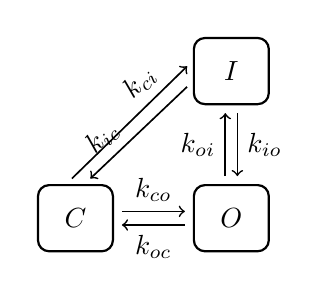
\begin{tikzpicture}[
   font=\sffamily,
   every matrix/.style={ampersand replacement=\&,column sep=1cm,row sep=1cm},
   state/.style={draw,thick,rounded corners,inner sep=.3cm},
   to/.style={->,semithick,shorten >=0.1cm,shorten <=0.1cm},
   Q/.style={->,semithick,sloped,pos=0.700000,shorten >=0.1cm,shorten <=0.1cm},  
   every node/.style={auto}]
\matrix{
\&\node[state] (I) {\parbox{10pt}{\centerline{$I$}}};\\
\node[state] (C) {\parbox{10pt}{\centerline{$C$}}};\&\node[state] (O) {\parbox{10pt}{\centerline{$O$}}};\\
};
\draw[to]  (O.100) to node {$k_{oi}$} (I.260);
\draw[to]  (O.190) to node {$k_{oc}$} (C.350);
\draw[to]  (I.280) to node {$k_{io}$} (O.80);
\draw[Q]  (I.195) to node {$k_{ic}$} (C.75);
\draw[to]  (C.10) to node {$k_{co}$} (O.170);
\draw[Q]  (C.105) to node {$k_{ci}$} (I.165);
\end{tikzpicture}
\end{center}
\caption{Markov model including three possible states: open (O), closed (C), and
inactivated (I).}%
\label{Ionchannels_L/ICO.pdf}%
\end{figure}


%\fig[0.5]{Ionchannels_L/ICO.pdf}{Markov model including three possible states; open (O),  closed (C) and inactivated (I).}

\subsection{Equilibrium probabilities}

We saw above (see page \pageref{eq_prob_ioc}) that the  equilibrium state of the
reaction shown in Figure  \ref{Ionchannels_L/ICO.pdf} is given by
\begin{align*}
o  &  =\frac{1}{1+\frac{k_{oc}}{k_{co}}+\frac{k_{oi}}{k_{io}}},\\
c  &  =\frac{\frac{k_{oc}}{k_{co}}}{1+\frac{k_{oc}}{k_{co}}+\frac{k_{oi}%
}{k_{io}}},\\
i  &  =\frac{\frac{k_{oi}}{k_{io}}}{1+\frac{k_{oc}}{k_{co}}+\frac{k_{oi}%
}{k_{io}}}.
\end{align*}


These probabilities are graphed as functions of the transmembrane potential in Figure
\ref{V/eq.pdf}. Note that the open probability in equilibrium is quite small; the channel is basically closed
for $v$ close to zero and it is inactivated for large values of $v$.

\fig{V/eq.pdf}{Equilibrium probabilities of the open, closed, and inactivated states as functions of the transmembrane potential $v$.}



\section{Probability density functions in the presence of the inactivated
state \label{pdfi}}

When the inactivated state is included in the model, as indicated in Figure  \ref{Ionchannels_L/ICO.pdf},
 the system governing the associated probability density functions is given by%
\begin{align}
\frac{\partial\rho_{o}}{\partial t}+\frac{\partial}{\partial v}\left(
a_{o}\rho_{o}\right)   &  =k_{co}\rho_{c}-(k_{oc}+k_{oi})\rho_{o}+k_{io}%
\rho_{i},\label{vpdfi1}\\
\frac{\partial\rho_{c}}{\partial t}+\frac{\partial}{\partial v}\left(
a_{c}\rho_{c}\right)   &  =k_{oc}\rho_{o}-(k_{co}+k_{ci})\rho_{c}+k_{ic}%
\rho_{i},\label{vpdfi2}\\
\frac{\partial\rho_{i}}{\partial t}+\frac{\partial}{\partial v}\left(
a_{c}\rho_{i}\right)   &  =k_{oi}\rho_{o}-(k_{io}+k_{ic})\rho_{i}+k_{ci}%
\rho_{c}\label{vpdfi3},
\end{align}
where
\begin{align}
a_{o}  &  =-g_{L}\left(  v-V_{L}\right)  -(v-V_{i})=\frac{11}{10}\left(
1-v\right)  ,\label{vfluxi}\\
a_{c}  &  =-g_{L}\left(  v-V_{L}\right)  =-\frac{1}{10}v.\nonumber
\end{align}


\subsection{Numerical simulations}
Again, we want to compare the solution computed by Monte Carlo simulations based on the stochastic
differential equation given in (\ref{v1b}) and the probability density functions defined by the system  (\ref{vpdfi1})--(\ref{vpdfi3}).
The numerical results are given in their usual form in Figure \ref{V/ioc.pdf}. 
As expected, the histograms computed using Monte Carlo simulations
and the numerical solution of the system  (\ref{vpdfi1})--(\ref{vpdfi3}) are quite similar. In these computations, 
the stochastic simulation ran for 100 s, with $\Delta t=0.01$ ms, and we used the mesh size $\Delta v=0.01$ in the numerical solution of the system  (\ref{vpdfi1})--(\ref{vpdfi3}). It is particularly interesting to
see that the tiny boundary layer close to $v=0$ for the probability density function of the inactivated state is captured using both the Monte Carlo and the probability density function approaches.


\fig{V/ioc.pdf}{Probability density functions of the open, closed, and inactivated states
(red lines) computed as numerical solutions of the system (\ref{vpdfi1})--(\ref{vpdfi3}) and
histograms based on Monte Carlo simulations using the stochastic differential
equation (\ref{v1b}). 
%{\bf xxx Glenn: is this the stationary solution of the pde?}. \G{yes.}
}


\section[Mutations affecting inactivation]{Mutations affecting the inactivated state of the ion channel\label{mutaffectinactiv}}

Certain mutations of the sodium channel are known to impair the
channel's ability to deactivate. We introduce a mutation severity index $\mu$
and assume that the reaction rates of the mutant are changed such that both
the probabilities of moving from the inactivated to the closed state and from the 
inactivated to the open state are increased. The effect of these changes will clearly be to lower 
the probability of the channel being in the inactivated state.

In mathematical terms, we define%
\begin{align}
\bar{k}_{ic} &  =\mu k_{ic},\label{ratesvm}\\
\bar{k}_{io} &  =\mu k_{io}, \nonumber
\end{align}
where $\mu\geqslant1$ and where $k_{ic}$ and $k_{io}$ are the wild type
reaction rates given by $\left(  \ref{ratesv}\right)  .$ It should be noted that the
new reaction rates still satisfy the principle of detailed balance. 
%\K{zzz Jeg er litt usikker p\r{a} hva som menes med den forrige setningen.
%$k_{io}$ forandres ikke, men $\bar{k}_{io}$ er jo ikke lik $k_{io}$.
%Er poenget at ''the principle of detailed balance'' fortsatt gjelder selv
%om vi bruker $\bar{k}_{ic}$ og $\bar{k}_{io}$ i stedet for $k_{ic}$ og $k_{io}$?}
% \A{Corrected}
In Figure \ref{V/mu_ioc.pdf}, we show the equilibrium
probability density functions of the open, closed, and inactivated states for 
the wild type and for three values of the mutation severity index $\mu.$

\fig{V/mu_ioc.pdf}{Probability density functions of the open, closed, and 
inactivated states for the wild type and for three values of the mutation 
severity index: $\mu=1.5,\, 3,\, 10.$ Larger values of $\mu$ give
solutions farther away from the wild type solution (solid line). The probability density of the closed state is 
only shown for $v$ between 0 and 0.1 to magnify very small differences.}



\section[Drug for mutations of inactivation]{A theoretical drug for mutations affecting the inactivation}


We want to derive a theoretical drug repairing the effect of the mutation described in (\ref{ratesvm}). In the Markov model
illustrated in Figure  \ref{Ionchannels_L/BICO.pdf}, we have introduced a blocked state associated with the open, closed, and inactivated state and
we now want to figure out what the best choice might be.
The equilibrium solution of the reaction represented in Figure \ref{Ionchannels_L/BICO.pdf} is characterized by the equations%
\begin{align*}
k_{co}c &  =k_{oc}o,\, k_{ci}c   =k_{ic}i,\\
k_{oi}o &  =k_{io}i,\, k_{bc}b_{c}   =k_{cb}c,\\
k_{bo}b_{o} &  =k_{ob}o, \, k_{bi}b_{i}   =k_{ib}i.
\end{align*}
It is useful to define%
\[
r_{xy}=\frac{k_{xy}}{k_{yx}}%
\]
and to note that%
\[
r_{xy}=\frac{1}{r_{yx}}.
\]
With this notation, the principle of detailed balance stating that%
\[
\frac{k_{co}k_{oi}k_{ic}}{k_{oc}k_{io}k_{ci}}=1
\]
can be written as%
\[
r_{co}r_{oi}r_{ic}=r_{oc}r_{io}r_{ci}=1.
\]
The equations above can now be written as%
\begin{align*}
c &  =r_{oc}o,\, c   =r_{ic}i,\\
o &  =r_{io}i,\, b_{c}   =r_{cb}c,\\
b_{o} &  =r_{ob}o,\, b_{i}   =r_{ib}i.
\end{align*}
It is convenient to express all probabilities in terms of the open probability:%
\begin{align*}
c &  =r_{oc}o,\\
i &  =r_{oi}o,\\
b_{c} &  =r_{cb}c=r_{cb}r_{oc}o,\\
b_{o} &  =r_{ob}o,\\
b_{i} &  =r_{ib}i=r_{ib}r_{oi}o.
\end{align*}
Since $c+i+o+b_{c}+b_{o}+b_{i}=1,$ we have%
\[
o=p^{-1},%
\]
where%
\[
p    =1+r_{oc}\left(  1+r_{cb}\right)  +r_{oi}\left(  1+r_{ib}\right)  +r_{ob}.%
\]
We refer to $p$ as the inverse open probability and we note that for the wild type
it is given by%
\[
p=1+r_{oc}+r_{oi}.
\]

\begin{figure}[ptb]
\begin{center}
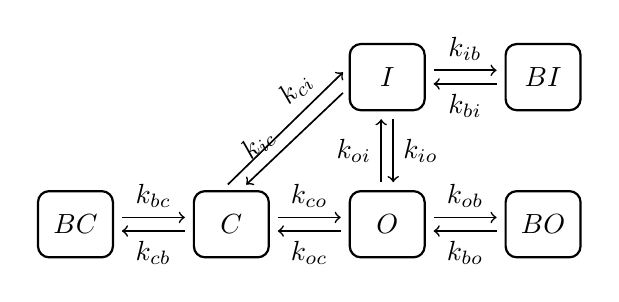
\begin{tikzpicture}[
   font=\sffamily,
   every matrix/.style={ampersand replacement=\&,column sep=1cm,row sep=1cm},
   state/.style={draw,thick,rounded corners,inner sep=.3cm},
   to/.style={->,semithick,shorten >=0.1cm,shorten <=0.1cm},
   Q/.style={->,semithick,sloped,pos=0.700000,shorten >=0.1cm,shorten <=0.1cm},  
   every node/.style={auto}]
\matrix{
\&\&\node[state] (I) {\parbox{10pt}{\centerline{$I$}}};\&\node[state] (BI) {\parbox{10pt}{\centerline{$BI$}}};\\
\node[state] (BC) {\parbox{10pt}{\centerline{$BC$}}};\&\node[state] (C) {\parbox{10pt}{\centerline{$C$}}};\&\node[state] (O) {\parbox{10pt}{\centerline{$O$}}};\&\node[state] (BO) {\parbox{10pt}{\centerline{$BO$}}};\\
};
\draw[to]  (O.100) to node {$k_{oi}$} (I.260);
\draw[to]  (O.190) to node {$k_{oc}$} (C.350);
\draw[to]  (O.10) to node {$k_{ob}$} (BO.170);
\draw[to]  (I.280) to node {$k_{io}$} (O.80);
\draw[Q]  (I.195) to node {$k_{ic}$} (C.75);
\draw[to]  (I.10) to node {$k_{ib}$} (BI.170);
\draw[to]  (C.10) to node {$k_{co}$} (O.170);
\draw[Q]  (C.105) to node {$k_{ci}$} (I.165);
\draw[to]  (C.190) to node {$k_{cb}$} (BC.350);
\draw[to]  (BO.190) to node {$k_{bo}$} (O.350);
\draw[to]  (BI.190) to node {$k_{bi}$} (I.350);
\draw[to]  (BC.10) to node {$k_{bc}$} (C.170);
\end{tikzpicture}
\end{center}
\caption{The model represented in Figure \ref{Ionchannels_L/ICO.pdf} extended 
to account for blockers associated with the closed state (BC), 
the open state (BO), and inactivated state (BI).}
\label{Ionchannels_L/BICO.pdf}
\end{figure}

%\fig[0.7]{Ionchannels_L/BICO.pdf}{The model represented in Figure \ref{Ionchannels_L/ICO.pdf} extended to account for 
%blockers associated the closed state (BC), the open state (O) and the inactivated state (BI).}

\subsection{Open probability in the mutant case }

As discussed above, we are interested in understanding how to define a
theoretical drug for mutations affecting the inactivation of the ion channel.
 We assume that the mutation affects the inactivation in a way that reduces the
probability of being in the inactivated state.  As mentioned above, this can be modeled by increasing
the reaction rates from the inactivated state to both the closed and the open states. We assume that
\[
\bar{k}_{ic}=\mu k_{ic},\text{ }\bar{k}_{io}=\mu k_{io},%
\]
where $\mu\geqslant1$ is the mutation severity index.
This gives%
\[
\bar{r}_{ic}=\frac{\bar{k}_{ic}}{k_{ci}}=\mu r_{ic}%
\]
and%
\[
\bar{r}_{io}=\frac{\bar{k}_{io}}{k_{oi}}=\mu r_{io}.
\]
We assume that the reaction rates between the closed and open states are
unaffected by the mutation and therefore%
\[
\bar{r}_{oc}=r_{oc}.
\]
Detailed balance dictates that we should have
\[
(\mu k_{ic}) k_{co} k_{oi} = (\mu k_{io}) k_{oc} k_{ci},
\] 
which holds regardless of the choice of $\mu$, since the wild type rates satisfy the
principle of detailed balance.

The inverse open probability in the presence of the mutations is given by%
\[
\bar{p}=1+r_{oc}+\bar{r}_{oi}=1+r_{oc}+1/\bar{r}_{io} =1+r_{oc}+\frac{1}{\mu r_{io}}
 = 1+r_{oc}+\frac{r_{oi}}{\mu}.
\]

%%%%%%%%%%%%%%%%%%%%%%%%%%%%%%%%%%%%%%%%%%%

\subsection{The open probability in the presence of the theoretical drug}

When the drug given in Figure \ref{Ionchannels_L/BICO.pdf} is applied, the inverse open probability is%
\[
p_{b}=1+r_{oc}\left(  1+r_{cb}\right)  +\frac{r_{oi}}{\mu}\left(
1+r_{ib}\right)  +r_{ob}%
\]
where $r_{cb},r_{ib}$, and $r_{ob}$ are used to characterize the drug. Our aim
is to now use these parameters to tune the drug such that%
\[
p_{b}\approx p,
\]
where $p$ is the inverse open probability of the wild type. More precisely, we
want to determine the constants $r_{cb},r_{ib}$, and $r_{ob}$ such that
\[
1+r_{oc}\left(  1+r_{cb}\right)  +\frac{r_{oi}}{\mu}\left(  1+r_{ib}\right)
+r_{ob}\approx1+r_{oc}+r_{oi}%
\]
holds for all relevant values of the transmembrane potential $v.$ We observe
that if we put $r_{cb}=r_{ob}=0,$ we obtain the condition%
\[
\frac{r_{oi}}{\mu}\left(  1+r_{ib}\right)  \approx r_{oi}%
\]
and therefore we set%
\[
r_{ib}=\mu-1.
\]
We conclude that we can repair the equilibrium state of the mutation
completely by applying a drug consisting of a blocker of the inactivated
state, provided that the reaction rates of the drug satisfy%
\[
\frac{k_{ib}}{k_{bi}}=\mu-1,
\]
where $\mu$ is the severity index of the mutation. This means that we have
reduced the problem of finding a drug to a single parameter given by
$k_{bi}.$ This remaining degree of freedom will be addressed below.


\section[PDFs: blocked inactivated state]{Probability density functions using the blocker of the inactivated state}

\begin{figure}[ptb]
\begin{center}
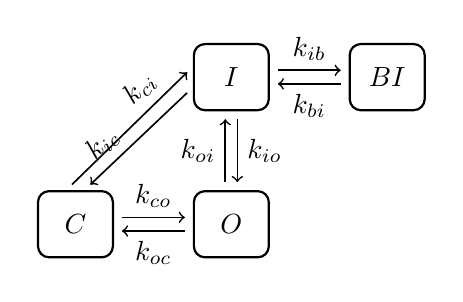
\begin{tikzpicture}[
   font=\sffamily,
   every matrix/.style={ampersand replacement=\&,column sep=1cm,row sep=1cm},
   state/.style={draw,thick,rounded corners,inner sep=.3cm},
   to/.style={->,semithick,shorten >=0.1cm,shorten <=0.1cm},
   Q/.style={->,semithick,sloped,pos=0.700000,shorten >=0.1cm,shorten <=0.1cm},  
   every node/.style={auto}]
\matrix{
\&\node[state] (I) {\parbox{10pt}{\centerline{$I$}}};\&\node[state] (BI) {\parbox{10pt}{\centerline{$BI$}}};\\
\node[state] (C) {\parbox{10pt}{\centerline{$C$}}};\&\node[state] (O) {\parbox{10pt}{\centerline{$O$}}};\&\\
};
\draw[to]  (O.100) to node {$k_{oi}$} (I.260);
\draw[to]  (O.190) to node {$k_{oc}$} (C.350);
\draw[to]  (I.280) to node {$k_{io}$} (O.80);
\draw[Q]  (I.195) to node {$k_{ic}$} (C.75);
\draw[to]  (I.10) to node {$k_{ib}$} (BI.170);
\draw[to]  (C.10) to node {$k_{co}$} (O.170);
\draw[Q]  (C.105) to node {$k_{ci}$} (I.165);
\draw[to]  (BI.190) to node {$k_{bi}$} (I.350);
\end{tikzpicture}
\end{center}
\caption{Markov model of the prototype ion channel with a blocker associated with the inactivated state.}
\label{Ionchannels_L/BICO4.pdf}
\end{figure}



%\fig[0.7]{Ionchannels_L/BICO4.pdf}{Markov model of the prototype ion channel with a blocker associated with the inactivated state.}

In Section \ref{pdfi} above, we derived a system governing the probability density
functions of the open, closed, and inactivated states. Here, we want to extend
the system to account for the theoretical drug represented by a blocker of the
inactivated state. The Markov model of the drug is given in Figure \ref{Ionchannels_L/BICO4.pdf}. The drug will
completely repair the equilibrium state of the Markov model, provided that
\begin{equation}
k_{ib}=\left(  \mu-1\right)  k_{bi}\label{kib},%
\end{equation}
where $\mu$ is the mutation severity index of the mutation (see (\ref{ratesvm})). The
stationary probability density functions of the states in the Markov model of
Figure \ref{Ionchannels_L/BICO4.pdf} are governed by the system%
\begin{align}
\frac{\partial}{\partial v}\left(  a_{o}\rho_{o}\right)   &  =k_{co}\rho
_{c}-\left(  k_{oc}+ k_{oi}\right)  \rho_{o}+\mu k_{io}\rho
_{i},\label{bvpdfi1}\\
\frac{\partial}{\partial v}\left(  a_{c}\rho_{c}\right)   &  =k_{oc}\rho
_{o}-\left(  k_{co}+ k_{ci}\right)  \rho_{c}+\mu k_{ic}\rho
_{i},\label{bvpdfi2}\\
\frac{\partial}{\partial v}\left(  a_{c}\rho_{i}\right)   &  = k_{oi}\rho_{o}-(\mu k_{io}+\mu k_{ic}+\left(  \mu-1\right)  k_{bi})\rho_{i}%
+k_{ci}\rho_{c}+k_{bi}\rho_{b},\label{bvpdfi3}\\
\frac{\partial}{\partial v}\left(  a_{c}\rho_{b}\right)   &  =\left(
\mu-1\right)  k_{bi}\rho_{i}-k_{bi}\rho_{b},\label{bvpdfi4}%
\end{align}
%\K{zzz Jeg forst\r{a}r ikke hvorfor man her deler $k_{oi}$ og $k_{ci}$ p\r{a}
%$\mu$ i stedet for \r{a} gange $k_{io}$ og $k_{ic}$ med $\mu$.}
%\A{Error. Background: we played with different directions for the mutation. Fixed now. xxx Glenn: Make sure code act according to corrected text}
%\G{The code has the mutation in the correct place, as in (11.6).}
where $\rho_{o},\rho_{c},\rho_{i},$ and $\rho_{b}$ denote the probability density
functions of the open, closed, inactivated, and blocked states, respectively, 
and where the flux terms are given by
\begin{align*}
a_{o} &  =-g_{L}\left(  v-V_{L}\right)  -(v-V_{i})=\frac{11}{10}\left(
1-v\right)  ,\\
a_{c} &  =-g_{L}\left(  v-V_{L}\right)  =-\frac{1}{10}v.
\end{align*}
The associated model of the wild type is given by%
\begin{align}
\frac{\partial}{\partial v}\left(  a_{o}\rho_{o}\right)   &  =k_{co}\rho
_{c}-\left(  k_{oc}+k_{oi}\right)  \rho_{o}+k_{io}\rho_{i},\label{pdf100}\\
\frac{\partial}{\partial v}\left(  a_{c}\rho_{c}\right)   &  =k_{oc}\rho
_{o}-\left(  k_{co}+k_{ci}\right)  \rho_{c}+k_{ic}\rho_{i},\label{pdf101}\\
\frac{\partial}{\partial v}\left(  a_{c}\rho_{i}\right)   &  =k_{oi}\rho
_{o}-(k_{io}+k_{ic})\rho_{i}+k_{ci}\rho_{c}.\label{pdf102}%
\end{align}
All the reactions rates used in the computations are given in (\ref{ratesv}); the computational domain
is given by $\Omega=[0,1]$ and we used 201 mesh points. 
In Figure \ref{V/drug_ico.pdf}, we show the difference between the open state probability density
function of the wild type, denoted by $\rho_{o},$ computed by solving the
system ($\ref{pdf100}$)--($\ref{pdf102}$), and the mutant where the
drug is applied, computed by solving ($\ref{bvpdfi1}$)--($\ref{bvpdfi4}$), denoted by $\rho_{o}^{\ast}.$ The difference is defined by the norm%
\begin{equation}
\Vert  \rho_{o}-\rho_{o}^{\ast}\Vert=\frac{\left\Vert \rho_{o}-\rho_{o}^{\ast}\right\Vert _{L^{2}\left(
\Omega\right)  }}{\left\Vert \rho_{o}\right\Vert _{L^{2}\left(  \Omega\right)
}+\left\Vert \rho_{o}^{\ast}\right\Vert _{L^{2}\left(  \Omega\right)  }}, \label{normfrac}%
\end{equation}
where, as usual,%
\[
\left\Vert \rho\right\Vert _{L^{2}\left(  \Omega\right)  }=\left(
\int_{\Omega}\rho^{2}dv\right)  ^{1/2}.
\]
We observe that, as $k_{bi}$ increases, the drug defined by $\left(
\ref{kib}\right)  $ completely repairs the effect of the mutation.

\fig{V/drug_ico.pdf}{The difference between the open probability density function
of the wild type ($\rho$) and the open probability density function ($\rho^\ast$) of the mutant using the drug defined by
(\ref{kib}), measured by the norm $\Vert  \rho_{o}-\rho_{o}^{\ast}\Vert$ defined in  (\ref{normfrac}). The difference
goes to zero as the parameter $k_{bi}$ is increased.}



%\section{Notes}

%\begin{itemize}
%\item The functions and parameters of (\ref{ratesv}) is motivated by xxxGlenn: where did you get it? referencexxx. \G{Somewhat arbitrarily, st{\aa}r det n{\aa}. Det stemmer bra. Brukte muligens Clancy som inspirasjon, men ikke til aa kjenne igjen naa.}
%\end{itemize}
